\normaltrue
\correctionfalse

%\UPSTIidClasse{11} % 11 sup, 12 spé
%\newcommand{\UPSTIidClasse}{12}

\exer{Mouvement T -- $\star$ \label{CIN:01:B2:13:PTSI:01:02}}
\setcounter{question}{0}\marginnote{\xpComp{CIN}{01}}%\UPSTIcompetence[2]{B2-13}
\index{Compétence B2-13-PTSI}
\index{Mécanisme à 1 translation}
\ifcorrection
\else
\marginnote{\textbf{Pas de corrigé pour cet exercice.}}
\fi

\ifprof
\else ~\\
Soit le mécanisme suivant. On note $\vect{AB}=\lambda(t)\vect{i_0}$.
\begin{marginfigure}
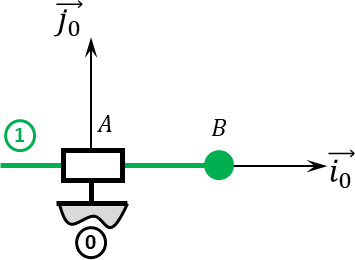
\includegraphics[width=\linewidth]{01_T_01}
\end{marginfigure}
\fi

\question{Réaliser le paramétrage du mécanisme.}
\ifprof ~\\

\else
\fi



\ifprof
\else
\footnotesize

\normalsize

\marginnote{Corrigé voir \ref{CIN:01:B2:13:PTSI:01:02}.}

\fi


